\documentclass[12pt]{scrartcl}

\usepackage{amsmath,amssymb}
\usepackage{fullpage}
\usepackage{enumitem}
\usepackage{hyperref}
\usepackage{graphicx}
\usepackage{tikz}
\usepackage{pgfplots}
\usepackage{float}
\usepackage{tabularx}
\usepackage{titlesec}

\pgfplotsset{compat=1.18}
\usetikzlibrary{trees,positioning,shapes,arrows}
\usepgfplotslibrary{statistics} 
\setlength{\parindent}{0pt}

\tikzset{
  basic/.style  = {draw, text width=2cm, drop shadow, font=\sffamily, rectangle},
  root/.style   = {basic, rounded corners=2pt, thin, align=center, fill=white},
  level-2/.style = {basic, rounded corners=6pt, thin,align=center, fill=white, text width=3cm},
  level-3/.style = {basic, thin, align=center, fill=white, text width=1.8cm}
}

\titleformat{\section}  % which section command to format
{\fontsize{12}{14}\bfseries} % format for whole line
{\thesection} % how to show number
{1em} % space between number and text
{} % formatting for just the text
[] % formatting for after the text

\titleformat{\subsection}  % which section command to format
{\fontsize{12}{14}\bfseries} % format for whole line
{\thesubsection} % how to show number
{1em} % space between number and text
{} % formatting for just the text
[] % formatting for after the text

\begin{document}

\begin{center}
	\hrule
	\vspace{0.4cm}
	{\textbf{\large Lecture 03: Discrete Probability Distributions}}\\ [0.2cm]
	INF1004 Mathematics II

\end{center}

\textbf{Name:} Timothy Chia \hspace{\fill} \textbf{Date:} 19/01/2025 \\

\hrule

\section{Random Variables \& Uncertainty}

\subsection{Variables vs. Random Variables}
To begin understanding probability models, we must first distinguish between standard algebraic variables and random variables. A variable is simply a symbol that represents some quantity without any inherent assumptions about its specific value. In contrast, a random variable is a value that strictly follows a probability distribution, meaning its eventual outcome is subject to randomness or chance. By standard mathematical convention, a random variable is denoted by a capital letter, such as $X$, while a lowercase letter, such as $x$, represents the specific numerical value it can assume during an observation.

\subsection{Discrete Random Variables}
A discrete random variable is characterised by its ability to take on one of a countable list of distinct, separate values. Because the possible outcomes are distinct jumps rather than a continuous spectrum, we are able to mathematically calculate exact probabilities for specific, individual outcomes.

\begin{figure}[h]
\centering
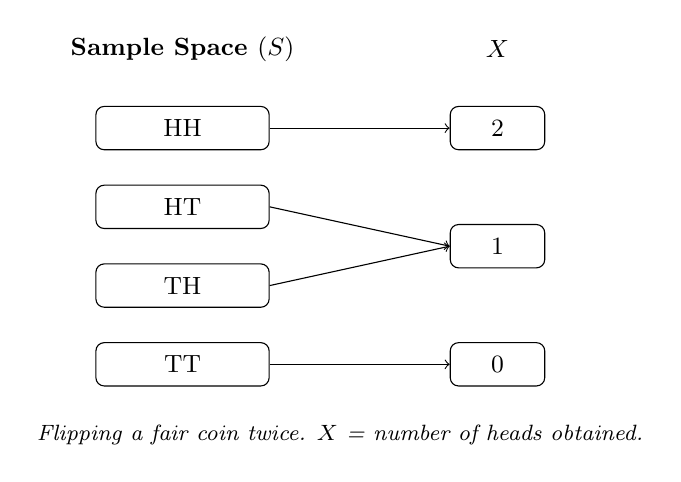
\begin{tikzpicture}[
    outcome/.style={draw, rounded corners=3pt, minimum width=2.2cm,
                    minimum height=0.55cm, align=center, font=\small},
    rv/.style={draw, rounded corners=3pt, minimum width=1.2cm,
               minimum height=0.55cm, align=center, font=\small},
    lbl/.style={font=\small\bfseries}
]
 
% --- Column headers ---
\node[lbl] at (0, 3.5)  {Sample Space $(S)$};
\node[lbl] at (4, 3.5)  {$X$};
 
% --- Left column: outcomes ---
\node[outcome] (HH) at (0,  2.5) {HH};
\node[outcome] (HT) at (0,  1.5) {HT};
\node[outcome] (TH) at (0,  0.5) {TH};
\node[outcome] (TT) at (0, -0.5) {TT};
 
% --- Right column: RV values ---
\node[rv] (X2) at (4,  2.5) {$2$};
\node[rv] (X1) at (4,  1.0) {$1$};
\node[rv] (X0) at (4, -0.5) {$0$};
 
% --- Arrows ---
\draw[->] (HH.east) -- (X2.west);
\draw[->] (HT.east) -- (X1.west);
\draw[->] (TH.east) -- (X1.west);
\draw[->] (TT.east) -- (X0.west);

% --- Caption ---
\node[font=\footnotesize\itshape, align=center] at (2, -1.4)
    {Flipping a fair coin twice. $X$ = number of heads obtained.};
 
\end{tikzpicture}
\caption{Mapping of random event outcomes to a discrete random variable.}
\end{figure}

\newpage
\subsection{Continuous Random Variables}
Conversely, a continuous random variable can take any value within a defined interval or collection of intervals. Because of this infinite continuity and lack of gaps between possible numbers, we are mathematically limited to finding probabilities for intervals or ranges of values rather than exact, single points in space or time.

\begin{figure}[h]
\centering
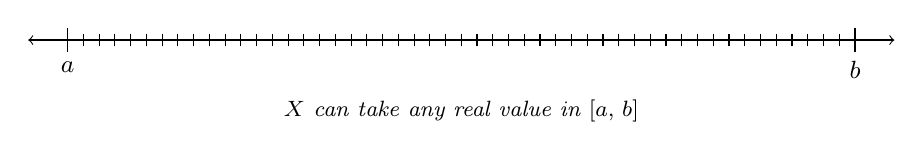
\begin{tikzpicture}
 
% --- Number line ---
\draw[<->] (-0.5, 0) -- (10.5, 0);
 
% --- Endpoints ---
\foreach \x/\lbl in {0/a, 10/b} {
    \draw (\x, -0.15) -- (\x, 0.15);
    \node[below, font=\small] at (\x, -0.15) {$\lbl$};
}
 
% --- Dense tick marks to suggest infinitely many points ---
\foreach \x in {
    0.2, 0.4, 0.6, 0.8, 1.0, 1.2, 1.4, 1.6, 1.8, 2.0,
    2.2, 2.4, 2.6, 2.8, 3.0, 3.2, 3.4, 3.6, 3.8, 4.0,
    4.2, 4.4, 4.6, 4.8, 5.0, 5.2, 5.4, 5.6, 5.8, 6.0,
    6.2, 6.4, 6.6, 6.8, 7.0, 7.2, 7.4, 7.6, 7.8, 8.0,
    8.2, 8.4, 8.6, 8.8, 9.0, 9.2, 9.4, 9.6, 9.8
} {
    \draw (\x, -0.08) -- (\x, 0.08);
}
 
% --- Caption ---
\node[font=\footnotesize\itshape, align=center] at (5, -0.9)
    {$X$ can take any real value in $[a,\, b]$};
 
\end{tikzpicture}
\caption{A continuous random variable represented on a 1D number line.}
\end{figure}

\section{Discrete Probability Distributions}
The probability distribution of a discrete random variable $X$ is defined as the comprehensive collection of all possible values $x$ along with their mathematically associated probabilities. For a discrete probability distribution to be mathematically valid, it must strictly adhere to two core rules. First, the probability of any exact outcome must logically lie between 0 and 1 inclusive, which is expressed mathematically as:

\[
0 \le P(X=x) \le 1
\]

Second, the sum of all probabilities for every possible outcome in the entire distribution must equal exactly 1, written as:

\[
\sum{P(X=x)=1}
\]

\begin{figure}[h]
\centering
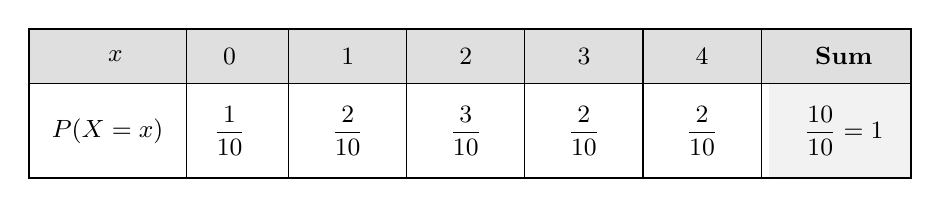
\begin{tikzpicture}[font=\small]
 
% Column positions
\def\colA{0}
\def\colB{2.2}
\def\colC{3.7}
\def\colD{5.2}
\def\colE{6.7}
\def\colF{8.2}
\def\colG{9.7}  % Sum column
 
% Row geometry
% Header row: y = 0 to 0.7  (centre at 0.35)
% Data row:   y = -1.2 to 0 (centre at -0.6)
%   taller data row gives fractions breathing room
\def\tableW{11.2}
 
% Header row background
\fill[gray!25] (0, 0) rectangle (\tableW, 0.7);
 
% Data row background (Sum cell slightly shaded)
\fill[gray!10] (9.4, -1.2) rectangle (\tableW, 0);
 
% Outer border
\draw[thick] (0, -1.2) rectangle (\tableW, 0.7);
 
% Internal vertical lines
\foreach \x in {2.0, 3.3, 4.8, 6.3, 7.8, 9.3} {
    \draw (\x, -1.2) -- (\x, 0.7);
}
 
% Horizontal line between header and data
\draw (0, 0) -- (\tableW, 0);
 
% Header labels (centred in 0 to 0.7)
\node at (1.1,  0.35) {$x$};
\node at (2.55, 0.35) {$0$};
\node at (4.05, 0.35) {$1$};
\node at (5.55, 0.35) {$2$};
\node at (7.05, 0.35) {$3$};
\node at (8.55, 0.35) {$4$};
\node at (10.35, 0.35) {\textbf{Sum}};
 
% Data row labels (centred in -1.2 to 0, i.e. at -0.6)
\node at (1.0,  -0.6) {$P(X=x)$};
\node at (2.55, -0.6) {$\dfrac{1}{10}$};
\node at (4.05, -0.6) {$\dfrac{2}{10}$};
\node at (5.55, -0.6) {$\dfrac{3}{10}$};
\node at (7.05, -0.6) {$\dfrac{2}{10}$};
\node at (8.55, -0.6) {$\dfrac{2}{10}$};
\node[font=\small\itshape] at (10.35, -0.6) {$\dfrac{10}{10} = 1$};
 
\end{tikzpicture}
\caption{A valid discrete probability distribution: all probabilities lie in $[0,1]$ and sum to~$1$.}
\end{figure}

\newpage
\subsection{Frequency vs. Probability}

It is helpful to note the conceptual difference between frequency distributions and probability distributions. While discrete data variables representing observed historical events are represented using a frequency distribution, discrete random variables representing uncertain future phenomena are described using probability distributions.

\begin{figure}[h]
\centering
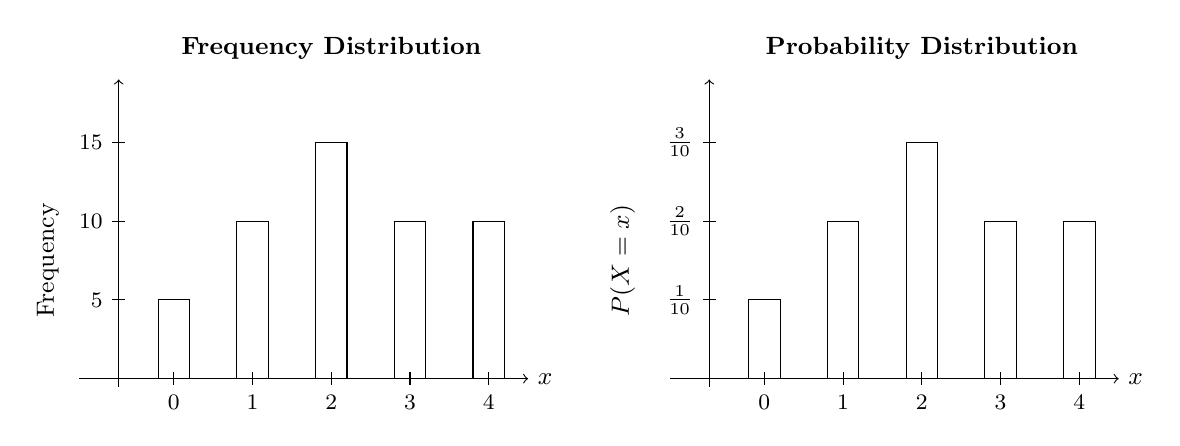
\begin{tikzpicture}[font=\small]
 
% ── LEFT CHART: Frequency Distribution ──────────────────────
 
% Axes
\draw[->] (-0.5, 0) -- (5.2, 0) node[right] {$x$};
\draw[->] (0, -0.1) -- (0, 3.8);
 
% y-axis ticks and labels  (freq * 0.2 = height in cm)
\draw (-0.08, 1.0) -- (0.08, 1.0);  \node[left,  font=\footnotesize] at (-0.08, 1.0) {5};
\draw (-0.08, 2.0) -- (0.08, 2.0);  \node[left,  font=\footnotesize] at (-0.08, 2.0) {10};
\draw (-0.08, 3.0) -- (0.08, 3.0);  \node[left,  font=\footnotesize] at (-0.08, 3.0) {15};
 
% y-axis label
\node[rotate=90, font=\small] at (-0.9, 1.5) {Frequency};
 
% Bars: x=0 -> freq 5 -> h=1.0,  x=1 -> 10 -> 2.0,  x=2 -> 15 -> 3.0,
%        x=3 -> 10 -> 2.0,  x=4 -> 10 -> 2.0
\draw (0.5,  0) rectangle (0.9,  1.0);
\draw (1.5,  0) rectangle (1.9,  2.0);
\draw (2.5,  0) rectangle (2.9,  3.0);
\draw (3.5,  0) rectangle (3.9,  2.0);
\draw (4.5,  0) rectangle (4.9,  2.0);
 
% x-axis ticks and labels
\foreach \xpos/\lbl in {0.7/0, 1.7/1, 2.7/2, 3.7/3, 4.7/4} {
    \draw (\xpos, -0.08) -- (\xpos, 0.08);
    \node[below, font=\footnotesize] at (\xpos, -0.08) {\lbl};
}
 
% Title
\node[font=\small\bfseries] at (2.7, 4.2) {Frequency Distribution};
 
% ── RIGHT CHART: Probability Distribution ───────────────────
 
\begin{scope}[xshift=7.5cm]
 
% Axes
\draw[->] (-0.5, 0) -- (5.2, 0) node[right] {$x$};
\draw[->] (0, -0.1) -- (0, 3.8);
 
% y-axis ticks and labels  (prob * 10 = height in cm)
% 1/10 -> 1.0cm,  2/10 -> 2.0cm,  3/10 -> 3.0cm
\draw (-0.08, 1.0) -- (0.08, 1.0);  \node[left, font=\footnotesize] at (-0.08, 1.0) {$\tfrac{1}{10}$};
\draw (-0.08, 2.0) -- (0.08, 2.0);  \node[left, font=\footnotesize] at (-0.08, 2.0) {$\tfrac{2}{10}$};
\draw (-0.08, 3.0) -- (0.08, 3.0);  \node[left, font=\footnotesize] at (-0.08, 3.0) {$\tfrac{3}{10}$};
 
% y-axis label
\node[rotate=90, font=\small] at (-1.1, 1.5) {$P(X=x)$};
 
% Bars: x=0 -> 1/10 -> h=1.0,  x=1 -> 2/10 -> 2.0,  x=2 -> 3/10 -> 3.0,
%        x=3 -> 2/10 -> 2.0,  x=4 -> 2/10 -> 2.0
\draw (0.5,  0) rectangle (0.9,  1.0);
\draw (1.5,  0) rectangle (1.9,  2.0);
\draw (2.5,  0) rectangle (2.9,  3.0);
\draw (3.5,  0) rectangle (3.9,  2.0);
\draw (4.5,  0) rectangle (4.9,  2.0);
 
% x-axis ticks and labels
\foreach \xpos/\lbl in {0.7/0, 1.7/1, 2.7/2, 3.7/3, 4.7/4} {
    \draw (\xpos, -0.08) -- (\xpos, 0.08);
    \node[below, font=\footnotesize] at (\xpos, -0.08) {\lbl};
}
 
% Title
\node[font=\small\bfseries] at (2.7, 4.2) {Probability Distribution};
 
\end{scope}
 
\end{tikzpicture}
\caption{Frequency distribution (observed counts) vs.\ probability distribution (uncertain outcomes) using the same underlying data.}
\end{figure}

\section{Expected Value and Measuring Spread}

\subsection{Expected Value (Mean)}

When analysing a discrete random variable, we often want to summarise its overall behavior. The mean, or expected value, of a discrete random variable is found by multiplying each possible value by its corresponding probability and subsequently adding the whole lot together. The mathematical formula for the expected value is:

\[
E(X) = \mu = \sum{[x  \cdot P(X=x)]}
\]

\subsection{Law of Large Numbers}
The practical, real-world importance of the expected value is highlighted by the \textit{Law of Large Numbers}. This statistical law states that as the number of independent trials increases, the mean outcome of those cumulative trials will gradually tend to become equal to the theoretical expected value.

\begin{figure}[H]
\centering
\begin{tikzpicture}
\begin{axis}[
    width=0.85\textwidth,
    height=6.5cm,
    xlabel={Number of trials},
    ylabel={Mean outcome},
    title={Convergence of Sample Mean to Expected Value (Fair Die, 1000 Trials)},
    xmin=1, xmax=1000,
    ymin=1, ymax=6,
    grid=both,
    grid style={dotted, gray!50},
    legend pos=north east,
    legend style={font=\small},
    tick label style={font=\small},
    label style={font=\small},
    title style={font=\small},
]
 
% Running mean from CSV
\addplot[black, thin] table[col sep=comma, x=trial, y=mean]{lln_data.csv};
\addlegendentry{Running mean}
 
% Expected value dashed line
\addplot[black, dashed, domain=1:1000, samples=2] {3.5};
\addlegendentry{Expected value ($\mu = 3.5$)}
 
\end{axis}
\end{tikzpicture}
\caption{As the number of independent trials increases, the running mean converges toward the theoretical expected value $\mu = 3.5$.}
\end{figure}

\subsection{Variance}
To understand the spread or dispersion of the possible data points away from the expected value, we calculate the variance. The variance of a discrete random variable $X$ measures the weighted average of the squared deviations from the mean. It is calculated using the formula:

\[
Var(X) = \sigma^{2} = \sum{[(x - \mu)^2 \cdot P(X = x)]}
\]

\subsection{Standard Deviation}
While variance provides a mathematically useful measure of spread, it scales in squared units. The standard deviation corrects this by taking the square root of the variance, returning the measurement of spread back to the original units of the variable. It is simply expressed as:

\[
\sigma = \sqrt{\sigma^2}
\]

\subsection{Coefficient of Variation}
In scenarios where we need to compare the relative spread of different distributions—such as evaluating the comparative financial risk between two distinct investment plans—we can calculate the coefficient of variation. By dividing the standard deviation by the mean, this formula provides a standardised measure of proportional dispersion:

\[
CV_{X} = \frac{\sigma_{X}}{\mu_{X}}
\]

% [Visual: Side-by-Side Bar Charts Comparing a Low Variance Distribution and a High Variance Distribution]
% Purpose: To illustrate how different data spreads look graphically despite potentially sharing the exact same expected value.

\begin{figure}[h]
\centering
 
% ── LEFT: Low Variance ───────────────────────────────────────
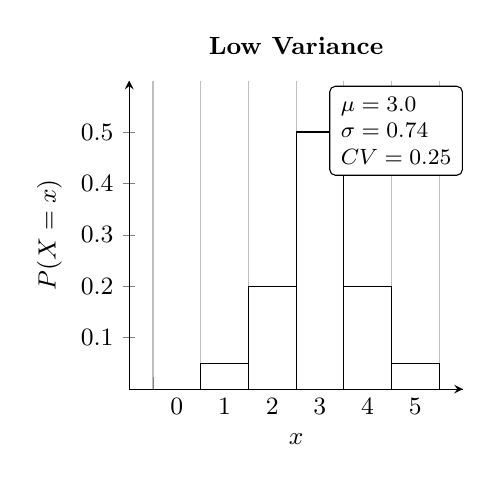
\begin{tikzpicture}
\begin{axis}[
    width=0.48\textwidth,
    height=5.5cm,
    title={\textbf{Low Variance}},
    xlabel={$x$},
    ylabel={$P(X=x)$},
    ymin=0, ymax=0.6,
    xtick={0,1,2,3,4,5,6},
    xticklabels={0,1,2,3,4,5,6},
    ytick={0.1,0.2,0.3,0.4,0.5},
    ybar interval=1,
    bar width=0.4cm,
    tick label style={font=\small},
    label style={font=\small},
    title style={font=\small},
    axis lines=left,
    xmin=-0.5, xmax=6.5,
    xtick align=inside,
]
\addplot[fill=white, draw=black] coordinates {
    (0, 0.00)
    (1, 0.05)
    (2, 0.20)
    (3, 0.50)
    (4, 0.20)
    (5, 0.05)
    (6, 0.00)
    (7, 0.00)
};
\node[draw, rounded corners=2pt, fill=white, font=\footnotesize, align=left,
     inner sep=4pt, anchor=north east] at (axis cs:6.5, 0.59)
    {$\mu = 3.0$\\$\sigma = 0.74$\\$CV = 0.25$};
\end{axis}
\end{tikzpicture}
\hspace{0.01\textwidth}
% ── RIGHT: High Variance ─────────────────────────────────────
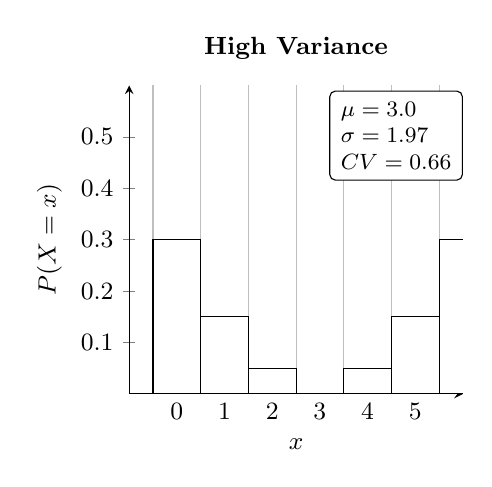
\begin{tikzpicture}
\begin{axis}[
    width=0.48\textwidth,
    height=5.5cm,
    title={\textbf{High Variance}},
    xlabel={$x$},
    ylabel={$P(X=x)$},
    ymin=0, ymax=0.6,
    xtick={0,1,2,3,4,5,6},
    xticklabels={0,1,2,3,4,5,6},
    ytick={0.1,0.2,0.3,0.4,0.5},
    ybar interval=1,
    bar width=0.4cm,
    tick label style={font=\small},
    label style={font=\small},
    title style={font=\small},
    axis lines=left,
    xmin=-0.5, xmax=6.5,
    xtick align=inside,
]
\addplot[fill=white, draw=black] coordinates {
    (0, 0.30)
    (1, 0.15)
    (2, 0.05)
    (3, 0.00)
    (4, 0.05)
    (5, 0.15)
    (6, 0.30)
    (7, 0.00)
};
\node[draw, rounded corners=2pt, fill=white, font=\footnotesize, align=left,
     inner sep=4pt, anchor=north east] at (axis cs:6.5, 0.59)
    {$\mu = 3.0$\\$\sigma = 1.97$\\$CV = 0.66$};
\end{axis}
\end{tikzpicture}
 
\caption{Two distributions sharing the same expected value ($\mu = 3.0$) but with markedly different spreads. The coefficient of variation $CV = \sigma/\mu$ captures this difference in a single standardised measure.}
\end{figure}

\section{Binomial Random Variables}

\subsection{Binomial Distributions}
A binomial random variable is a highly practical and special class of discrete random variables used to efficiently model specific types of recurring scenarios. 

A random phenomenon can be appropriately modeled as a binomial distribution if it strictly exhibits four defining features:
\begin{enumerate}
    \item The experiment must consist of a \textbf{finite number of identical trials}. 
    \item Each individual trial must result in \textbf{exactly one of two possible discrete outcomes}, conventionally labeled as "success" or "failure".
    \item The probability of success, denoted as $p$, and the probability of failure, calculated as $1 − p$, \textbf{must remain completely constant} from trial to trial.
    \item The outcomes must be completely independent, meaning \textbf{the result of one trial does not logically or physically influence the outcome of the next}.
\end{enumerate}

When all conditions are met, the probability distribution is written in the standard notation:
\[
X \sim B(n,p)
\]
where $n$ represents the total number of identical trials and $p$ represents the constant probability of success in a single trial.

\newpage
\subsection{Binomial Probability Formula}
The precise probability of achieving exactly $x$ successes across the $n$ trials can be efficiently calculated using the binomial probability formula. This allows us to bypass drawing massive probability trees. The formula is:

\[
P(X = x) = {n \choose x} \cdot p^{x} \cdot (1 - p)^{n-x}
\]

\subsection{Combinations}
Within the binomial formula, the "\textit{n choose x}" combinations factor determines the mathematical number of distinct ways the specified number of successes can be arranged across the trials. This combinatorial element is calculated using factorials as:

\[
{n \choose x} = C_{x}^{n} = \frac{n!}{(n - x)! \cdot x!}
\]

% [Visual: A Probability Tree Diagram Demonstrating the Combinations of Outcomes for 3 Independent Coin Flips]
% Purpose: To visually show the origin of the combinations multiplier and how individual permutations group together into distinct combination counts.


\begin{figure}[h]
\centering
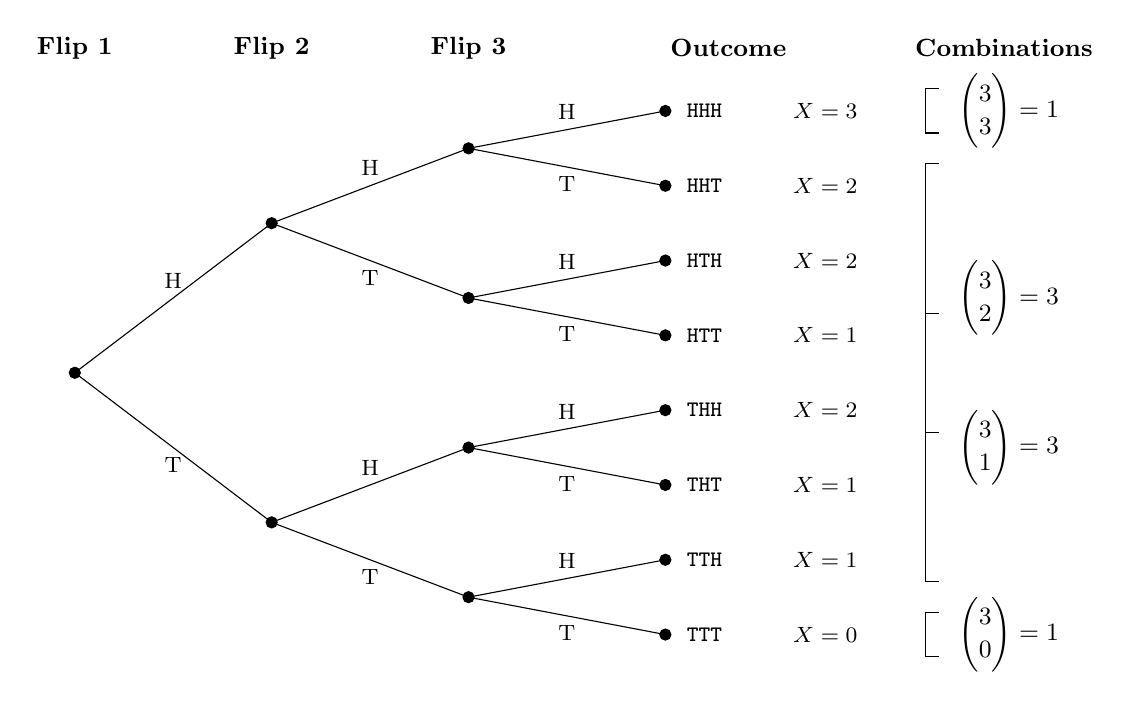
\begin{tikzpicture}[font=\small]
 
% ── Leaf y-values (cm, step 0.95) ────────────────────────────
\def\ya{7.60}  % HHH  X=3
\def\yb{6.65}  % HHT  X=2
\def\yc{5.70}  % HTH  X=2
\def\yd{4.75}  % HTT  X=1
\def\ye{3.80}  % THH  X=2
\def\yf{2.85}  % THT  X=1
\def\yg{1.90}  % TTH  X=1
\def\yh{0.95}  % TTT  X=0
 
% ── Internal node y-values (midpoints) ───────────────────────
\def\yHH{7.125}  \def\yHT{5.225}
\def\yTH{3.325}  \def\yTT{1.425}
\def\yH{6.175}   \def\yT{2.375}
\def\yR{4.275}
 
% ── Edges with inline labels ─────────────────────────────────
\draw (1,\yR)   -- node[midway, above, font=\footnotesize] {H} (3.5,\yH);
\draw (1,\yR)   -- node[midway, below, font=\footnotesize] {T} (3.5,\yT);
 
\draw (3.5,\yH) -- node[midway, above, font=\footnotesize] {H} (6,\yHH);
\draw (3.5,\yH) -- node[midway, below, font=\footnotesize] {T} (6,\yHT);
\draw (3.5,\yT) -- node[midway, above, font=\footnotesize] {H} (6,\yTH);
\draw (3.5,\yT) -- node[midway, below, font=\footnotesize] {T} (6,\yTT);
 
\draw (6,\yHH)  -- node[midway, above, font=\footnotesize] {H} (8.5,\ya);
\draw (6,\yHH)  -- node[midway, below, font=\footnotesize] {T} (8.5,\yb);
\draw (6,\yHT)  -- node[midway, above, font=\footnotesize] {H} (8.5,\yc);
\draw (6,\yHT)  -- node[midway, below, font=\footnotesize] {T} (8.5,\yd);
\draw (6,\yTH)  -- node[midway, above, font=\footnotesize] {H} (8.5,\ye);
\draw (6,\yTH)  -- node[midway, below, font=\footnotesize] {T} (8.5,\yf);
\draw (6,\yTT)  -- node[midway, above, font=\footnotesize] {H} (8.5,\yg);
\draw (6,\yTT)  -- node[midway, below, font=\footnotesize] {T} (8.5,\yh);
 
% (edge labels are inline on the \draw commands above)
 
% ── Nodes ────────────────────────────────────────────────────
\foreach \px/\py in {
    1/\yR,
    3.5/\yH, 3.5/\yT,
    6/\yHH,  6/\yHT,  6/\yTH,  6/\yTT,
    8.5/\ya, 8.5/\yb, 8.5/\yc, 8.5/\yd,
    8.5/\ye, 8.5/\yf, 8.5/\yg, 8.5/\yh} {
    \filldraw (\px,\py) circle (2pt);
}
 
% ── Outcome labels and X values ──────────────────────────────
\foreach \py/\lbl/\xv in {
    \ya/HHH/3, \yb/HHT/2, \yc/HTH/2, \yd/HTT/1,
    \ye/THH/2, \yf/THT/1, \yg/TTH/1, \yh/TTT/0} {
    \node[right, font=\footnotesize\ttfamily] at (8.65, \py) {\lbl};
    \node[right, font=\footnotesize]          at (10.0, \py) {$X=\xv$};
}
 
% ── Combination brackets ─────────────────────────────────────
% All coordinates hardcoded in cm (no arithmetic macros).
%   pad = 0.28,  stub = 0.18,  bx = 11.8
%
%   X=3: HHH y=7.60  -> top=7.88, bot=7.32
%   X=2: HHT y=6.65 .. THH y=3.80 -> top=6.93, bot=3.52, mid=5.225
%   X=1: HTT y=4.75 .. TTH y=1.90 -> top=5.03, bot=1.62, mid=3.325
%   X=0: TTT y=0.95  -> top=1.23, bot=0.67
 
% X=3
\draw (11.8, 7.32) -- (11.8, 7.88);
\draw (11.8, 7.88) -- (11.98, 7.88);
\draw (11.8, 7.32) -- (11.98, 7.32);
\node[anchor=west, font=\small] at (12.1, 7.60) {$\dbinom{3}{3}=1$};
 
% X=2
\draw (11.8, 3.52) -- (11.8, 6.93);
\draw (11.8, 6.93) -- (11.98, 6.93);
\draw (11.8, 3.52) -- (11.98, 3.52);
\node[anchor=west, font=\small] at (12.1, 5.225) {$\dbinom{3}{2}=3$};
 
% X=1
\draw (11.8, 1.62) -- (11.8, 5.03);
\draw (11.8, 5.03) -- (11.98, 5.03);
\draw (11.8, 1.62) -- (11.98, 1.62);
\node[anchor=west, font=\small] at (12.1, 3.325) {$\dbinom{3}{1}=3$};
 
% X=0
\draw (11.8, 0.67) -- (11.8, 1.23);
\draw (11.8, 1.23) -- (11.98, 1.23);
\draw (11.8, 0.67) -- (11.98, 0.67);
\node[anchor=west, font=\small] at (12.1, 0.95) {$\dbinom{3}{0}=1$};
 
% ── Column headers ────────────────────────────────────────────
\def\hy{8.4}
\node[font=\small\bfseries] at (1.0,  \hy) {Flip 1};
\node[font=\small\bfseries] at (3.5,  \hy) {Flip 2};
\node[font=\small\bfseries] at (6.0,  \hy) {Flip 3};
\node[font=\small\bfseries] at (9.3,  \hy) {Outcome};
\node[font=\small\bfseries] at (12.8, \hy) {Combinations};
 
\end{tikzpicture}
\caption{Probability tree for 3 independent coin flips. Each path from root to leaf represents one outcome. Outcomes with the same number of heads ($X$) are grouped to show the origin of the combinations multiplier $\binom{n}{x}$.}
\end{figure}

\newpage
\subsection{Simplified Metrics}
By identifying a scenario as a binomial distribution, the complex summation calculations usually required for finding expected value and variance are drastically simplified. All prior calculation tables are replaced by elegant, direct equations. The mean of a binomial random variable is calculated straightforwardly as:

\[
E(X) = \mu \ np
\]

And the variance is found using:

\[
Var(X) = \sigma^{2} = np(1 - p) = npq 
\]

% [Visual: A Histogram Plot of a Binomial Distribution]
% Purpose: To provide a final, comprehensive look at the familiar bell-like shape and expected behavior of a properly modeled binomial distribution.

\begin{figure}[h]
\centering
\begin{tikzpicture}
\begin{axis}[
    width=0.85\textwidth,
    height=6.5cm,
    title={Binomial Distribution: $n = 20$,\ $p = 0.5$},
    xlabel={$x$ (number of successes)},
    ylabel={$P(X=x)$},
    ymin=0,
    xmin=-0.5, xmax=20.5,
    xtick={0,1,...,20},
    ybar, bar width=0.55cm,
    fill=white, draw=black,
    tick label style={font=\small},
    label style={font=\small},
    title style={font=\small},
    axis lines=left,
    enlarge x limits=0.02,
    ytick={0, 0.05, 0.10, 0.15, 0.20},
    yticklabels={$0$, $0.05$, $0.10$, $0.15$, $0.20$},
    ymax=0.22,
]
 
% Binomial bars from CSV
\addplot[fill=white, draw=black]
    table[col sep=comma, x=x, y=prob]{binomial_data.csv};
 
% Dashed vertical line at mu=10, drawn as a TikZ line inside axis coordinates
\draw[dashed, black] (axis cs:10, 0) -- (axis cs:10, 0.20);
 
% Stats box — top left, clear of the bars
\node[draw, rounded corners=2pt, fill=white, font=\footnotesize,
      align=left, inner sep=5pt, anchor=north west] at (axis cs:0, 0.215)
    {$\mu = np = 10$\\[2pt]
     $\sigma^2 = np(1-p) = 5$\\[2pt]
     $\sigma = 2.24$};
 
\end{axis}
 
\end{tikzpicture}
\caption{Histogram of the binomial distribution with $n = 20$ trials and $p = 0.5$. The dashed line marks the expected value $\mu = np = 10$.}
\end{figure}

\end{document}
